%課題研究レジュメテンプレート ver. 1.2

\documentclass[uplatex]{jsarticle}
\usepackage[top=20mm,bottom=20mm,left=20mm,right=20mm]{geometry}
\usepackage[T1]{fontenc}
\usepackage{txfonts}
\usepackage{wrapfig}
\usepackage[expert,deluxe]{otf}
\usepackage[dvipdfmx,hiresbb]{graphicx}
\usepackage[dvipdfmx]{hyperref}
\usepackage{pxjahyper}
\usepackage{secdot}

\makeatletter
  \renewcommand{\section}{%
    \if@slide\clearpage\fi
    \@startsection{section}{1}{\z@}%
    {\Cvs \@plus.5\Cdp \@minus.2\Cdp}% 前アキ
    {.5\Cvs \@plus.3\Cdp}% 後アキ
    %{\normalfont\Large\headfont\raggedright}}
    {\normalfont\raggedright}}

  \renewcommand{\subsection}{\@startsection{subsection}{2}{\z@}%
    {\Cvs \@plus.5\Cdp \@minus.2\Cdp}% 前アキ
    {.5\Cvs \@plus.3\Cdp}% 後アキ
    %{\normalfont\large\headfont}}
    {\normalfont}}

  \renewcommand{\subsubsection}{\@startsection{subsubsection}{3}{\z@}%
    {\Cvs \@plus.5\Cdp \@minus.2\Cdp}%
    {\z@}%
    %{\normalfont\normalsize\headfont}}
    {\normalfont}}
\makeatother
%ここから上を編集する必要はない.





\title{\vspace{-14mm}リツイートユーザーリストとツイートの関係分析}
\author{PMコース 矢吹研究室 1442014 岩橋瑠伊}
\date{}%日付を入れる必要はない.
\pagestyle{empty}%ページ番号は振らない.
\begin{document}
\maketitle





\section{研究の背景}
今日SNSは,コミュニケーションプラットフォームとして,私たちにとって大変身近な存在になっている.同時にどのSNSにビジネスの可能性があるかなどの注目も集まっており,それぞれのSNS利用者数やアクティブユーザーの数は様々な調査データによって公表されている.
そのSNSの中からTwitterを選び,Twitterによるビジネスをより良くする手法について考えていく\cite{sns}.

Twitterは2006年7月15日に開設された「ツイート」と称される140文字以内の短文の投稿を共有するウェブ上の情報サービスである.2015年12月時点で,1カ月間Twitterにログインしたアクティブユーザー数は3500万人である.また,世界全体では3億2000万人で約1割が日本国内からのアクセスである\cite{twitter}.

Twitterでは,ツイートをすると自分のフォロワーの見ているタイムラインに自分のツイートが表示される.逆に,自分がフォローしている人がツイートをすると自分のタイムラインにそのツイートが表示される.その他のTwitterの機能にリツイートというものがあり,元のツイート者のユーザー名のまま,自分のフォロワーの見ているタイムラインに転送する仕組みである.この機能を使うことで自分が興味深い,拡散したいと思ったツイートを自分のフォロワーに伝えることが可能になる.

私はリツイートされて自分のタイムラインに表示されるツイートを見ていると,たまにリツイートしたユーザーの特徴と,リツイートされたツイートの特徴が一致しない場合があることに気が付いた.そこで,ツイートの条件によって発言者が想定したユーザーではないユーザーにリツイートが行われているのではないかと考えた.このことから,どのような条件のツイートなら,そのツイートの内容に関係したユーザーに多くリツイートされるのかを明らかにできるのではないかと考えた.

\section{研究の目的}

ツイート内容,公式アカウントであるか非公式アカウントであるか,フォローフォロワー数等の条件変化の下で,ツイート内容と,リツイートユーザーのツイートの特徴の,相関の変化を明らかにする

\section{プロジェクトマネジメントとの関連}

ツイートの条件によりツイートの内容を伝えたいユーザーに範囲を定められるならば,Twitterで広告を行う企業にとってのステークホルダー・マネジメントになると考えられる.

\section{研究の方法}

最低100リツイート以上されているツイートを集め,そのツイートのリツイートユーザーの中からTwitterAPIを利用して100人(TwitterAPI制限の限界値)のユーザーIDとScreanNameを取り出す.

取得した100人のユーザー全員の最新500ツイート(対象ユーザーの総ツイート数が500に満たない場合は対象ユーザーの全てのツイート)をTwitterAPIで取得する.


取得した100人のユーザーのそれぞれ500ツイートをまとめてMeCabで形態素解析を行い,文章中に含まれる名詞に関してtf-idfで重み付けをするスクリプトを実行する.


これにより抽出された名詞をチェックしていき,一つでもリツイートされたツイートの内容と関連する名詞が確認された場合,そのユーザーはリツイートされたツイートの内容と関係があると判断する.


\section{現在の進捗状況}

現在3つのツイートに関して手法の通り分析をし終えており,1つのツイートに関しては分析中である.

分析し終えた3つのツイートは図1のとおりである.図1の左側のツイートから得られた結果を説明していく.企業の公式アカウントが発信するその企業に関連した広告や告知ツイートは100人中80人関係があるという結果となった.図1の真ん中は企業の公式アカウントではないが,一般のユーザーがある企業の情報等を紹介しているツイートの場合100人中62人関係があるという結果となった.

この分析結果より,企業の公式アカウントによる企業の広告や告知はその企業の公式アカウントのフォロワーの種類の時点でユーザーが想定内に定まっていることが分かった.企業の公式アカウントであるという影響力によって,拡散されてもその企業の内容とユーザーが大きな相関を保っていると考えられる.また,一般のユーザーによる企業の紹介ツイートの例では拡散されていると言ってもあくまで一般のユーザーであり,公式アカウントとしての影響力には程遠い.一般のユーザーは企業の公式アカウントと違い情報の告知や宣伝のためではなく,一般のユーザー視点で興味を持ったユーザーをフォローしていく.その為,拡散されたツイートの内容に相関のないユーザーも多く巻き込んで拡散された結果,それなりの相関となったと考えられる.

図1の右側の結果は100人中6人関係があるという結果となった.

珍しい現象が見られるといったような内容は詳しくその現象について知らなかったとしてもツイートを見た瞬間にリツイートしがち(私がTwitterを利用した際の経験談から)であるということと,そのアカウントが提供する情報が多岐に渡るという点から様々な種類のフォロワーがそのアカウントにいると推測されるため低い関係性に繋がったのではないかと考えた.

\begin{figure}[h]
\centering
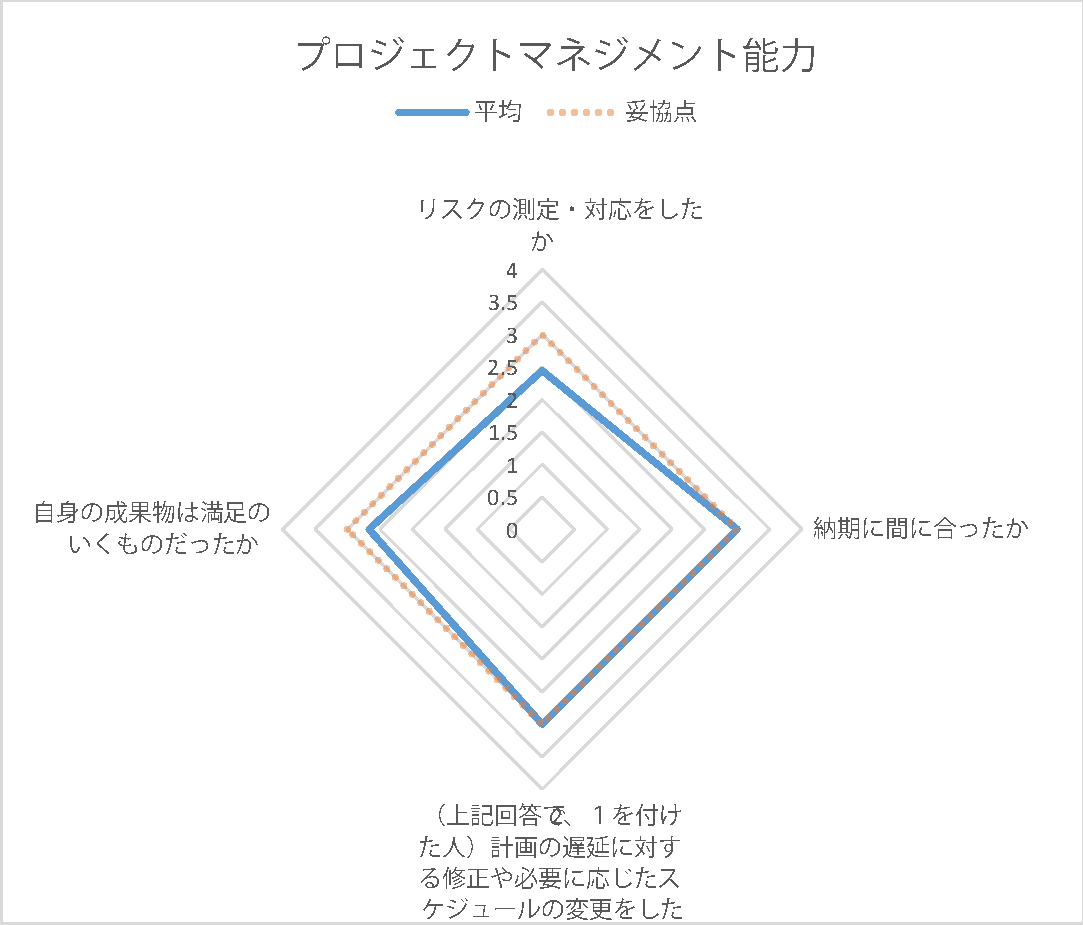
\includegraphics[width=15cm]{g1.pdf}
\caption{分析した3つのツイート}\label{ツイート}
\end{figure}

\section{今後の計画}
\begin{enumerate}
\item まだデータの数が少ないので多くのツイートを分析していくことで仮説検証を行う.
\item 様々な条件のツイートを分析することで新たな仮説を発見する.
\end{enumerate}

\bibliographystyle{junsrt}
\bibliography{biblio}%「biblio.bib」というファイルが必要.

\end{document}
